% !TEX TS-program = pdflatex
% !TEX encoding = UTF-8 Unicode

\documentclass[a4paper, titlepage=false, parskip=full-, 10pt]{scrartcl}

\usepackage[utf8]{inputenc}
\usepackage[T1]{fontenc}
\usepackage[english, ngerman]{babel}
\usepackage{babelbib}
\usepackage{hyperref}
\usepackage{listings}
\usepackage{framed}
\usepackage{color}
\usepackage{graphicx}
\usepackage[normalem]{ulem}
\usepackage{cancel}
\usepackage{array}
\usepackage{amsmath}
\usepackage{amssymb}
\usepackage{amsthm}
\usepackage{algorithm}
\usepackage{algorithmic}
\usepackage{geometry}
\usepackage{subfigure}
\geometry{a4paper, top=20mm, left=35mm, right=25mm, bottom=40mm}

\newcounter{tasknbr}
\setcounter{tasknbr}{1}
\newenvironment{task}[1]{{\bf Aufgabe \arabic {tasknbr}\stepcounter{tasknbr}} (#1):\begin{enumerate}}{\end{enumerate}}
\newcommand{\subtask}[1]{\item[#1)]}

% Listings -----------------------------------------------------------------------------
\definecolor{red}{rgb}{.8,.1,.2}
\definecolor{blue}{rgb}{.2,.3,.7}
\definecolor{lightyellow}{rgb}{1.,1.,.97}
\definecolor{gray}{rgb}{.7,.7,.7}
\definecolor{darkgreen}{rgb}{0,.5,.1}
\definecolor{darkyellow}{rgb}{1.,.7,.3}
\lstloadlanguages{C++,[Objective]C,Java}
\lstset{
escapeinside={§§}{§§},
basicstyle=\ttfamily\footnotesize\mdseries,
columns=fullflexible,
keywordstyle=\bfseries\color{blue},
commentstyle=\color{darkgreen},      
stringstyle=\color{red},
numbers=left,
numberstyle=\ttfamily\scriptsize\color{gray},
breaklines=true,
showstringspaces=false,
tabsize=4,
captionpos=b,
float=htb,
frame=tb,
frameshape={RYR}{y}{y}{RYR},
rulecolor=\color{black},
xleftmargin=15pt,
xrightmargin=4pt,
aboveskip=\bigskipamount,
belowskip=\bigskipamount,
backgroundcolor=\color{lightyellow},
extendedchars=true,
belowcaptionskip=15pt}

%% Enter current values here: %%
\newcommand{\lecture}{Robotik WS15/16}
\newcommand{\tutor}{}
\newcommand{\assignmentnbr}{13}
\newcommand{\students}{Julius Auer, Thomas Tegethoff}
%%-------------------------------------%%

\begin{document}  
{\small \textsl{\lecture \hfill \tutor}}
\hrule
\begin{center}
\textbf{Übungsblatt \assignmentnbr}\\
[\bigskipamount]
{\small \students}
\end{center}
\hrule

\begin{task}{}
\item[]
Wir messen hierfür die $x$-Position des Blocks $x^m$ via \emph{/ackerman\_vehicle/laser/scan/ranges$\left[269\right]+0.5$} (blau in Abbildung \ref{fig:1}) sowie die erste Ableitung davon $v^m$ (rot in Abbildung \ref{fig:1}). Außerdem messen wir die ''echten'' Werte $x^{gt},v^{gt}$ aus der Gazebo Ground-Truth. Nach 250 Iterationen erhalten wir somit 250 Datenpunkte für den Fehler zwischen Messung und Ground-Truth $X=\{(x^{gt}_1-x^m_1,v^{gt}_1-v^m_1),...,(x^{gt}_{250}-x^m_{250},v^{gt}_{250}-v^m_{250})\}$ und können die Kovarianzmatrix $R$ für diesen Fehler ausrechnen:

\begin{align*}
\mu&=\frac{1}{250}\cdot\sum_{i=1}^{250}X_i\\
R&=\frac{1}{250}\cdot\begin{pmatrix}\sum_{i=1}^{250}((X_{i1}-\mu_1)\cdot (X_{i1}-\mu_1))&\sum_{i=1}^{250}((X_{i1}-\mu_1)\cdot (X_{i2}-\mu_))\\\sum_{i=1}^{250}((X_{i2}-\mu_2)\cdot (X_{i1}-\mu_1))&\sum_{i=1}^{250}((X_{i2}-\mu_2)\cdot (X_{i2}-\mu_2))\end{pmatrix}
\end{align*}

Nach einigen Durchläufen kommt bei uns im Mittel so etwas heraus wie:
$$R=\begin{pmatrix}0.01&0.001\\0.001&1\end{pmatrix}$$

\begin{figure}[!htpb]
\centering
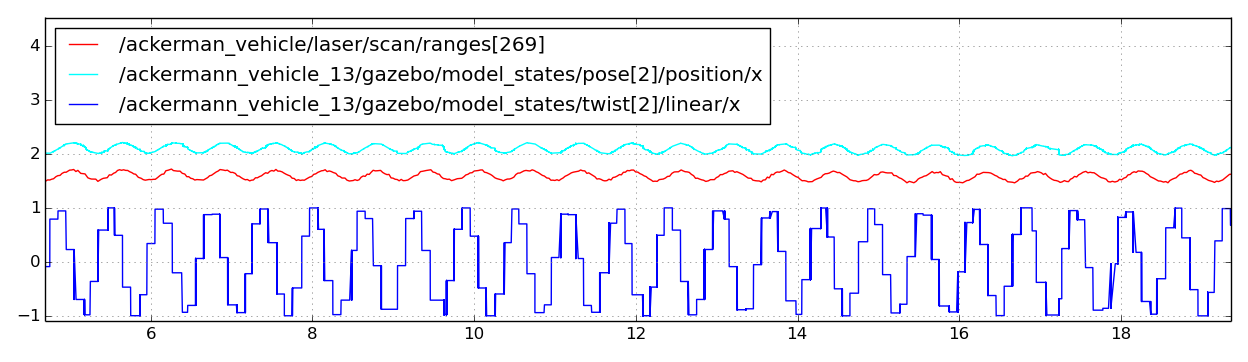
\includegraphics[width=1.1\linewidth]{capture_1-1}
\caption{Messungen und GT}
\label{fig:1}
\end{figure}
\end{task}

\newpage
\begin{task}{}
\item[]
Das geht so nicht: wir müssten hier als Fehler die Differenz zwischen der Gazebo-Ground-Truth Pose und $sin\left(\frac{2\cdot\pi\cdot t}{0.6}\right)$ berechnen. Das kann aber nur funktionieren, wenn wir $t$ genau kennen. Leider ist nicht angegeben, welche Zeit hier benutzt wird. Raten hilft nicht viel, da ROS, Gazebo und der gestartete Node alle unterschiedliche Timestamps ausgeben können. Auch die Einheit der Zeit ist somit nicht klar spezifiziert.

Das rauszukriegen wäre echt fummelig gewesen und wir haben - ehrlich gesagt - keinen Bock darauf. Wir haben immerhin in Aufgabe 1 gezeigt, dass wir grundsätzlich Fehler-Kovarianzmatrizen berechnen können, hier benutzen wir jetzt einfach:
$$Q=\begin{pmatrix}1&0\\0&1\end{pmatrix}$$
\end{task}

\begin{task}{}
\item[]
Joa. War nicht ganz einfach, ist aber eigentlich straight-forward:

Wir speichern stets die letzte Position und Geschwindigkeit $x$ und die letzte Kovarianzmatrix $p$. Immer wenn das Laser-Callback zum Zeitpunkt $t$ triggert updaten wir diese Werte wie folgt:

Measure:
\begin{align*}
m&=\begin{pmatrix}x^m_t\\v^m_t\end{pmatrix}
\end{align*}

Predict:
\begin{align*}
x'&=A\cdot x\\
p'&=A\cdot p\cdot A^T+Q
\end{align*}

Update:
\begin{align*}
k&=p'\cdot H^T\cdot (H\cdot p'\cdot H^T+R)\\
x&=x'+k\cdot (m-H\cdot x')\\
p&=p'-k\cdot H\cdot p'
\end{align*}

Ergebnisse zeigt Abbildung \ref{fig:3}. Wenn die Messdaten quasi perfekt sind, ist das Filtern natürlich ziemlich sinnlos. Für zukünftige Übungszettel würde ich Daten empfehlen, die wenigstens etwas verrauscht sind. Die Geschwindigkeit lässt sich auch nicht gut filtern - das System oszilliert zu schnell.

\begin{figure}[!htpb]
\centering
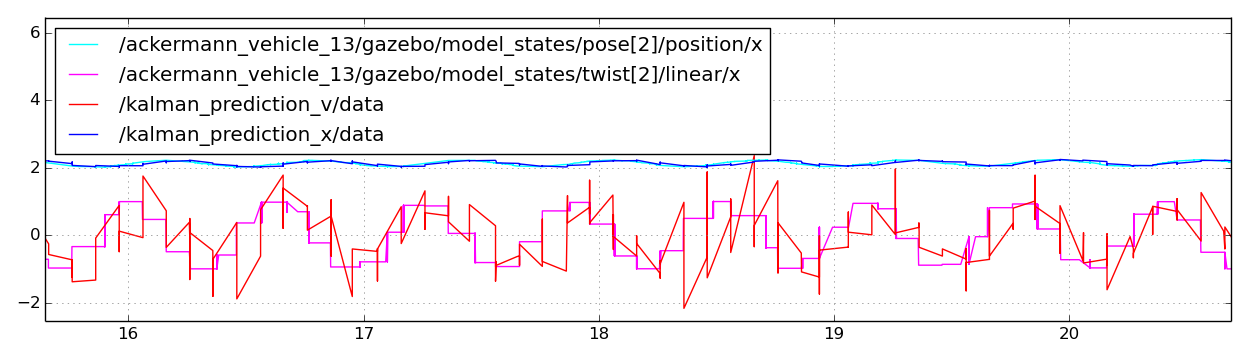
\includegraphics[width=1.1\linewidth]{capture_3-1}
\caption{Filter-Output und GT}
\label{fig:3}
\end{figure}
\end{task}
\end{document}